\documentclass[12pt]{report}
\usepackage{geometry}
\usepackage{graphicx}
\usepackage{amsmath}
\usepackage{hyperref}
\usepackage{fancyhdr}
\usepackage{setspace}
\usepackage{ragged2e}
\usepackage{listings}
\usepackage{xcolor}
\usepackage{sectsty}
\usepackage{lmodern}
\usepackage{tikz}
\usepackage{enumitem}
\usetikzlibrary{shapes,arrows,positioning,fit}
\usetikzlibrary{shapes.geometric, arrows}
\usetikzlibrary{shapes.geometric, arrows.meta, positioning}
\usetikzlibrary{shapes.geometric, arrows.meta}
\geometry{a4paper, total = {210mm, 297mm}, left=31.75mm, right=25.4mm, top=20.05mm, bottom=20.05mm}


\tikzstyle{startstop} = [rectangle, rounded corners, minimum width=4cm, minimum height=1cm, text centered, draw=black, fill=orange!30]
\tikzstyle{process} = [rectangle, minimum width=3cm, minimum height=1cm, text centered, draw=black, fill=orange!30]
\tikzstyle{arrow} = [thick,->,>=stealth]

\lstset{
  basicstyle=\ttfamily\footnotesize,
  keywordstyle=\color{blue},
  stringstyle=\color{red},
  commentstyle=\color{green},
  morekeywords={import, from},
  showstringspaces=false,
  breaklines=true
}
\lstset{
    language=Python,
    showstringspaces=false,
    frame=single,
    breaklines=true,
}

\sectionfont{\fontsize{18pt}{19.2pt}\selectfont}       % Chapter font size
\subsectionfont{\fontsize{16pt}{19.2pt}\selectfont} 
\subsubsectionfont{\fontsize{14pt}{16.8pt}\selectfont}

% Set margins
\geometry{a4paper, left=1.25in, right=1in, top=0.75in, bottom=0.75in}

% Page style setup
\pagestyle{fancy}
\fancyhf{} % Clear header and footer
\fancyhead[L]{\makebox[\textwidth][c]{\fontsize{10}{12}\selectfont REAL-TIME EMOTION DETECTION}}
\fancyfoot[L]{\fontsize{10}{12}\selectfont Department of ISE, CEC, Sudhindra Nagara, Benjanapadavu  2023-24}
\fancyfoot[R]{\thepage} % Page number at center footer
\makeatletter
\def\headrule{{%
    \color{brown}%
    \hrule width\headwidth height0.5pt \vskip1pt % Thin line
    \hrule width\headwidth height2pt \vskip-\headrulewidth % Thick line
    \vskip-3pt % Adjust space between lines and text
}}
\def\footrule{{%
    \color{brown}%
    \hrule width\headwidth height0.5pt \vskip1pt % Thin line
    \hrule width\headwidth height2pt \vskip-\footrulewidth % Thick line
    \vskip-3pt % Adjust space between lines and text
}}
\makeatother
\begin{document}
% Reset page style for subsequent pages
\pagenumbering{arabic}
% introduction
\newpage
\section*{CHAPTER 1}
\begin{center}
    \textbf{\fontsize{18pt}{21.6pt}\selectfont INTRODUCTION}  % Introduction font size
\end{center}
\vspace{0.2em}
\begin{center}    
    \setstretch{1.5} % Adjust line spacing
    \justify % Enable full justification
In today's digital age, the traditional methods of salary disbursement are increasingly being scrutinized for their inefficiencies and lack of transparency. The adoption of blockchain technology presents a transformative solution to these challenges. Blockchain, with its decentralized and immutable ledger, offers a secure and transparent method for managing financial transactions, making it an ideal candidate for modernizing payroll systems. \\
   Blockchain-based salary disbursement ensures that every transaction is securely recorded and easily verifiable, eliminating the risks of fraud and discrepancies. By automating payment processes through smart contracts, this technology streamlines operations and reduces administrative overhead. Employees benefit from real-time notifications and the assurance that their payments are processed accurately and on time. \\

 
\end{center}
\vspace{0.7em}
\subsection*{1.1 Motivation}
\begin{center}    
    \setstretch{1.5} % Adjust line spacing
    \justify % Enable full justification
Our project leverages these advantages by integrating Ethereum smart contracts with a robust backend developed in Flask and MongoDB for efficient data management. MetaMask is utilized for secure wallet interactions, providing a seamless and secure experience for both employers and employees. This innovative approach not only enhances the efficiency and security of salary disbursement but also fosters greater trust and transparency in financial transactions.
\end{center}
\subsection*{1.2 Contributions}
\begin{center}
\setstretch{1.5} % Adjust line spacing
    \justify
The salient contributions of this work are:
\begin{itemize}
	\setlength\itemsep{0.15em}
\item
Designed the overall system architecture, integrating blockchain technology with traditional web development frameworks to create a seamless salary disbursement platform.

\item  
Developed a user-friendly interface for admins and employees using web technologies.
\item
Implemented MetaMask for handling employee wallet addresses and transactions.
\item
Implemented MetaMask for handling employee wallet addresses and transactions.	
 \end{itemize}
 \end{center}
 \vspace{0.7em}
\subsection*{1.3 Report Outline}
\begin{center}    
    \setstretch{1.5} % Adjust line spacing
    \justify
This project report outlines the development and implementation of a blockchain-based salary disbursement system. The document begins with an introduction to the topic and the problem statement, followed by the purpose and scope of the project. It details the methodology used, including system requirements and software specifications. The report also covers the design and development of smart contracts, backend integration, and the implementation of security measures. Additionally, it includes testing procedures, results, and the overall impact of the system. Finally, the report concludes with insights, contributions, and future work.

\end{center}
%Literature Review
\newpage
\section*{CHAPTER 2}
\vspace{1EM}
\begin{center}
    \textbf{\fontsize{16pt}{21.6pt}\selectfont LITERATURE REVIEW}  % Introduction font size
\end{center}
\begin{center}    
    \setstretch{1.5} % Adjust line spacing
    \justify
Blockchain technology has revolutionized various industries by providing a decentralized and transparent system for managing transactions. Nakamoto's seminal paper on Bitcoin in 2008 introduced the concept of a blockchain, a distributed ledger that records transactions across multiple computers in such a way that the registered transactions cannot be altered retroactively. This innovation laid the foundation for numerous applications beyond cryptocurrencies, such as smart contracts, which are self-executing contracts with the terms of the agreement directly written into code. Smart contracts have been extensively explored in academic research and industry applications, showcasing their potential to automate processes, enhance security, and reduce the need for intermediaries. \\
In the realm of salary disbursement, traditional methods involve manual processing, significant paperwork, and intermediaries such as banks, which can lead to delays, errors, and increased costs. Recent studies highlight the inefficiencies and lack of transparency in these conventional systems. Blockchain technology offers a promising solution by enabling automated, secure, and transparent salary payments through smart contracts. Research indicates that implementing blockchain in salary disbursement can mitigate fraud, reduce transaction times, and ensure accurate and timely payments. Additionally, using blockchain enhances data security and integrity, as each transaction is cryptographically secured and immutable. This literature survey underscores the transformative potential of blockchain technology in creating more efficient and trustworthy systems for salary disbursement.
\end{center}
\vspace{0.7em}
\subsection*{2.1 Problem Statement}
\begin{center}    
    \setstretch{1.5} % Adjust line spacing
    \justify
 In traditional payroll systems, inefficiencies, lack of transparency, and security risks pose significant challenges for both employers and employees. These conventional methods often involve manual processes, are prone to errors, and can result in delayed payments, ultimately leading to mistrust and dissatisfaction among employees.
Traditional payroll systems face several challenges, including a lack of transparency that hinders real-time visibility into the disbursement process, potentially leading to discrepancies and mistrust. These systems are also susceptible to security risks, such as data breaches, fraud, and unauthorized access, which can compromise the confidentiality and integrity of financial transactions. Inefficiencies within these systems often result in delayed payments, negatively impacting employee morale and financial stability. Additionally, the manual handling of salary disbursements is both time-consuming and error-prone, increasing administrative overhead and the likelihood of mistakes.
\end{center}
\vspace{0.7em}
\subsection*{2.2 Objectives}
\begin{center}    
    \setstretch{1.5} % Adjust line spacing
    \justify
The objectives of this project are:
\begin{itemize}
    \item[$1)$] Enhance Transparency: Develop a system that ensures real-time visibility into salary disbursements, reducing discrepancies and building trust among employees and employers.
    \item[$2)$] Improve Security: Implement robust blockchain technology to safeguard financial transactions, reducing the risk of data breaches, fraud, and unauthorized access.
    \item[$3)$] Increase Efficiency: Automate salary disbursement processes to minimize delays, reduce administrative overhead, and decrease the likelihood of errors.
\end{itemize}
\end{center}
\vspace{0.7em}
\subsection*{2.3 Outcomes}
\begin{center}    
    \setstretch{1.5} % Adjust line spacing
    \justify
The outcomes of this salary disbursement with blockchain technology project are:
\begin{itemize}
    \subsection*{Increased Transparency}
    \item Achieved real-time visibility into salary disbursements, fostering greater trust and accountability.

    \subsection*{Enhanced Security}
    \item Strengthened the security of financial transactions through blockchain technology, minimizing the risk of fraud and data breaches.

    \subsection*{Reduced Administrative Overhead}
    \item Automated salary disbursement processes, significantly cutting down on manual tasks and administrative workload.

    \subsection*{Timely Payments}
    \item Ensured prompt and efficient salary payments, positively impacting employee satisfaction and financial stability.

    \subsection*{Accurate Record-Keeping}
    \item Maintained precise and tamper-proof records of all transactions, aiding in compliance and audit processes.

    \subsection*{Cost-Effective Solution}
    \item Lowered operational costs by reducing the need for intermediary services and manual processing.

    \subsection*{Scalability}
    \item Developed a scalable system capable of handling an increasing number of employees and transactions as the organization grows.
\end{itemize}

These outcomes demonstrate the significant advantages of integrating blockchain technology into salary disbursement systems. By enhancing transparency, security, and efficiency, the project successfully addressed key challenges in traditional payroll methods. The automation of processes and timely payments not only improved employee satisfaction but also reduced administrative overhead and operational costs. This scalable solution ensures accurate record-keeping and robust security, paving the way for future growth and innovation in financial transactions.
\end{center}

% system requirement specification
\newpage
\section*{CHAPTER 3}
\vspace{1EM}
\begin{center}
    \textbf{\fontsize{16pt}{21.6pt}\selectfont SOFTWARE REQUIREMENT SPECIFICATION}  % Introduction font size
\end{center}
\subsection*{3.1 Introduction}
\begin{center}    
    \setstretch{1.5} % Adjust line spacing
    \justify 
This Software Requirement Specification (SRS) outlines the requirements for the Salary disbursement application.
\end{center}
\vspace{0.7em}
\subsection*{3.2 Functional Requirements}
\begin{center}    
    \setstretch{1.5} % Adjust line spacing
    \justify 
\begin{enumerate}
    \item \textbf{User Authentication:} Secure login system for administrators to access the dashboard.
    \item \textbf{Employee Management:} Store and manage employee details including name, wallet address, salary amount, email, and employment status.
    \item \textbf{Salary Disbursement:} Automated disbursement of salaries using Ethereum smart contracts.
    \item \textbf{Transaction Management:} Store transaction details in MongoDB for auditability and transparency.
    \item \textbf{Notification System:}Send real-time email notifications to employees upon salary disbursement.
\end{enumerate}
\end{center}
\vspace{0.7em}
\subsection*{3.3 Non-Functional Requirements}
\begin{center}    
    \setstretch{1.5} % Adjust line spacing
    \justify 
\begin{enumerate}
    \item \textbf{Performance:} The system must efficiently handle salary disbursements and blockchain transactions without significant delays.
    \item \textbf{Usability:} The user interface should be intuitive and easy to navigate for both administrators and employees.
    \item \textbf{Reliability:} The system must ensure consistent uptime and accurate processing of all salary disbursements.
    \item \textbf{Scalability:} The system should be able to accommodate an increasing number of employees and transactions without compromising performance.
    \item \textbf{Compatibility:} The solution should be compatible with various web browsers and devices, providing a seamless user experience across different platforms.
\end{enumerate}
\end{center}
\vspace{0.7em}
\subsection*{3.4 Software Requirements}
\begin{center}    
    \setstretch{1.5} % Adjust line spacing
    \justify 
\begin{itemize}
    \item Operating System: Windows
    \item Frontend: Html,CSS,JavaScript
    \item Backend: Flask Framework Web3.py,Flask-Login,SMTP,Python Libraries
    \item Blockchain Integration: Hardhat,MetaMask
    \item Database: MongoDB
    \item Web Browser: Google Chrome
    \item Editor platform: Visual Studio Code 
\end{itemize}
\end{center}
\vspace{0.7em}
\subsection*{3.5 Hardware Requirements}
\begin{center}    
    \setstretch{1.5} % Adjust line spacing
    \justify 
\begin{itemize}
    \item Processor: Intel Core i5 (8th gen) or equivalent AMD processor
    \item RAM: 8 GB or higher
    \item Storage: 5 GB of free disk space
    \item Network Connection
\end{itemize}
\end{center}
\vspace{0.7em}
\subsection*{3.6 Constraints}
\begin{center}    
    \setstretch{1.5} % Adjust line spacing
    \justify 
\begin{itemize}
    \item Regulatory Compliance: The system must adhere to legal and regulatory standards for financial transactions and data privacy, which may vary depending on the jurisdiction.
    \item Scalability Limitations: The blockchain network's capacity and performance might impose limitations on the number of transactions and employees the system can efficiently handle.
    \item Integration Challenges: Ensuring seamless integration with existing systems, such as payroll software and email services, can be complex and may require additional development effort.
\end{itemize}
\end{center}

%Design
\newpage
\section*{CHAPTER 4}
\begin{center}
    \textbf{\fontsize{18pt}{21.6pt}\selectfont DESIGN}  % Introduction font size
\end{center}
\vspace{0.7em}
\subsection*{4.1 ARCHITECTURE DESIGN}
\begin{center}
 \setstretch{1.5} % Adjust line spacing
    \justify
The architectural design of the salary disbursement system leverages a multi-tiered approach to ensure robustness, scalability, and security. At the core of the architecture is the backend, which utilizes Flask for web development, MongoDB for data storage, and Hardhat with MetaMask for blockchain integration. This backend handles authentication, transaction processing, and interaction with the blockchain for salary disbursements. The frontend is built using HTML, CSS, and JavaScript, providing a user-friendly interface for administrators and employees to manage and view their payroll information. Integration with blockchain technology ensures transparent and secure salary payments, while the database schema efficiently stores employee details, transaction records, and system logs. Overall, the architecture is designed to support a scalable and secure system that meets the project’s functional and non-functional requirements.   
\end{center}
\vspace{1em}
\begin{figure}[h!]
\centering
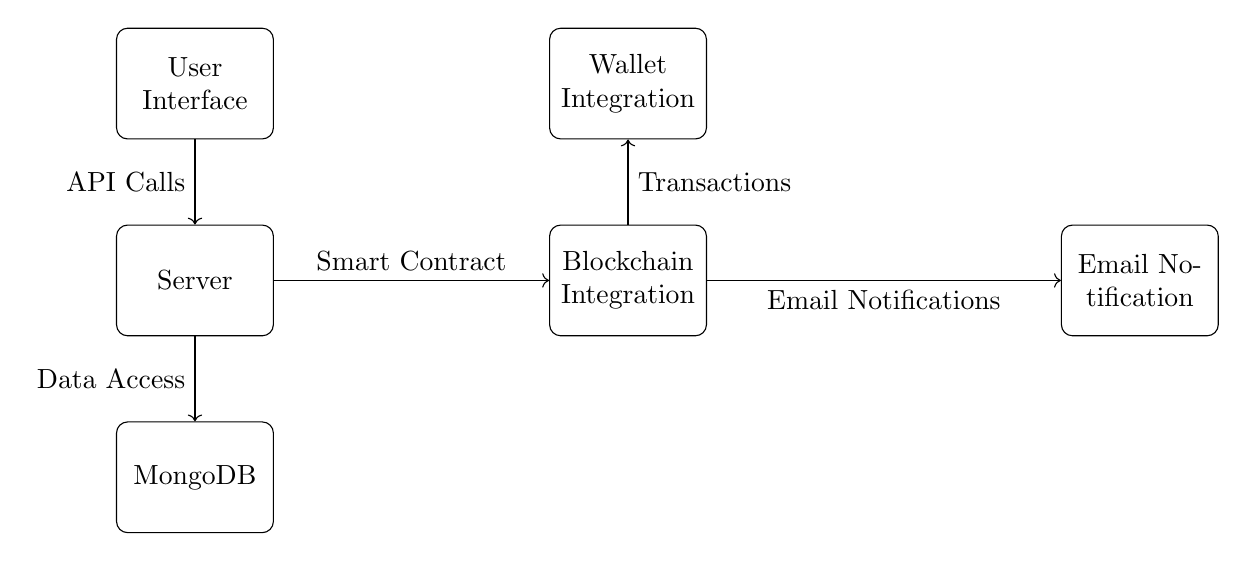
\begin{tikzpicture}[node distance=2.5cm and 4cm]
    \tikzstyle{block} = [rectangle, draw, fill=white!20, 
        text width=5em, text centered, rounded corners, minimum height=4em]
    \tikzstyle{line} = [draw, -latex']
    \node [block] (ui) {User Interface};
    \node [block](backend) [below of=ui] {Server};
    \node [block](blockchain) [ right of=backend, xshift=3cm] {Blockchain Integration};
    \node [block](database) [below of=backend] {MongoDB};
    \node [block](email) [right of=blockchain, xshift=4cm] {Email Notification};
    \node [block](wallet) [above of=blockchain] {Wallet Integration};

    % Arrows
    \draw[->] (ui) -- (backend) node[midway, left] {API Calls};
    \draw[->] (backend) -- (blockchain) node[midway, above] {Smart Contract};
    \draw[->] (backend) -- (database) node[midway, left] {Data Access};
    \draw[->] (blockchain) -- (email) node[midway, below] {Email Notifications};
    \draw[->] (blockchain) -- (wallet) node[midway, right] {Transactions};

    \end{tikzpicture}
\end{figure}
\begin{center}
    Figure 4.1.1 Architectural design of the Salary Disbursement System.
\end{center}
\newpage
\subsection*{4.2 DATA FLOW DIAGRAM}
\vspace{1em}
\textbf{LEVEL 0}
\vspace{0.5em}
\begin{figure}[h]
\centering
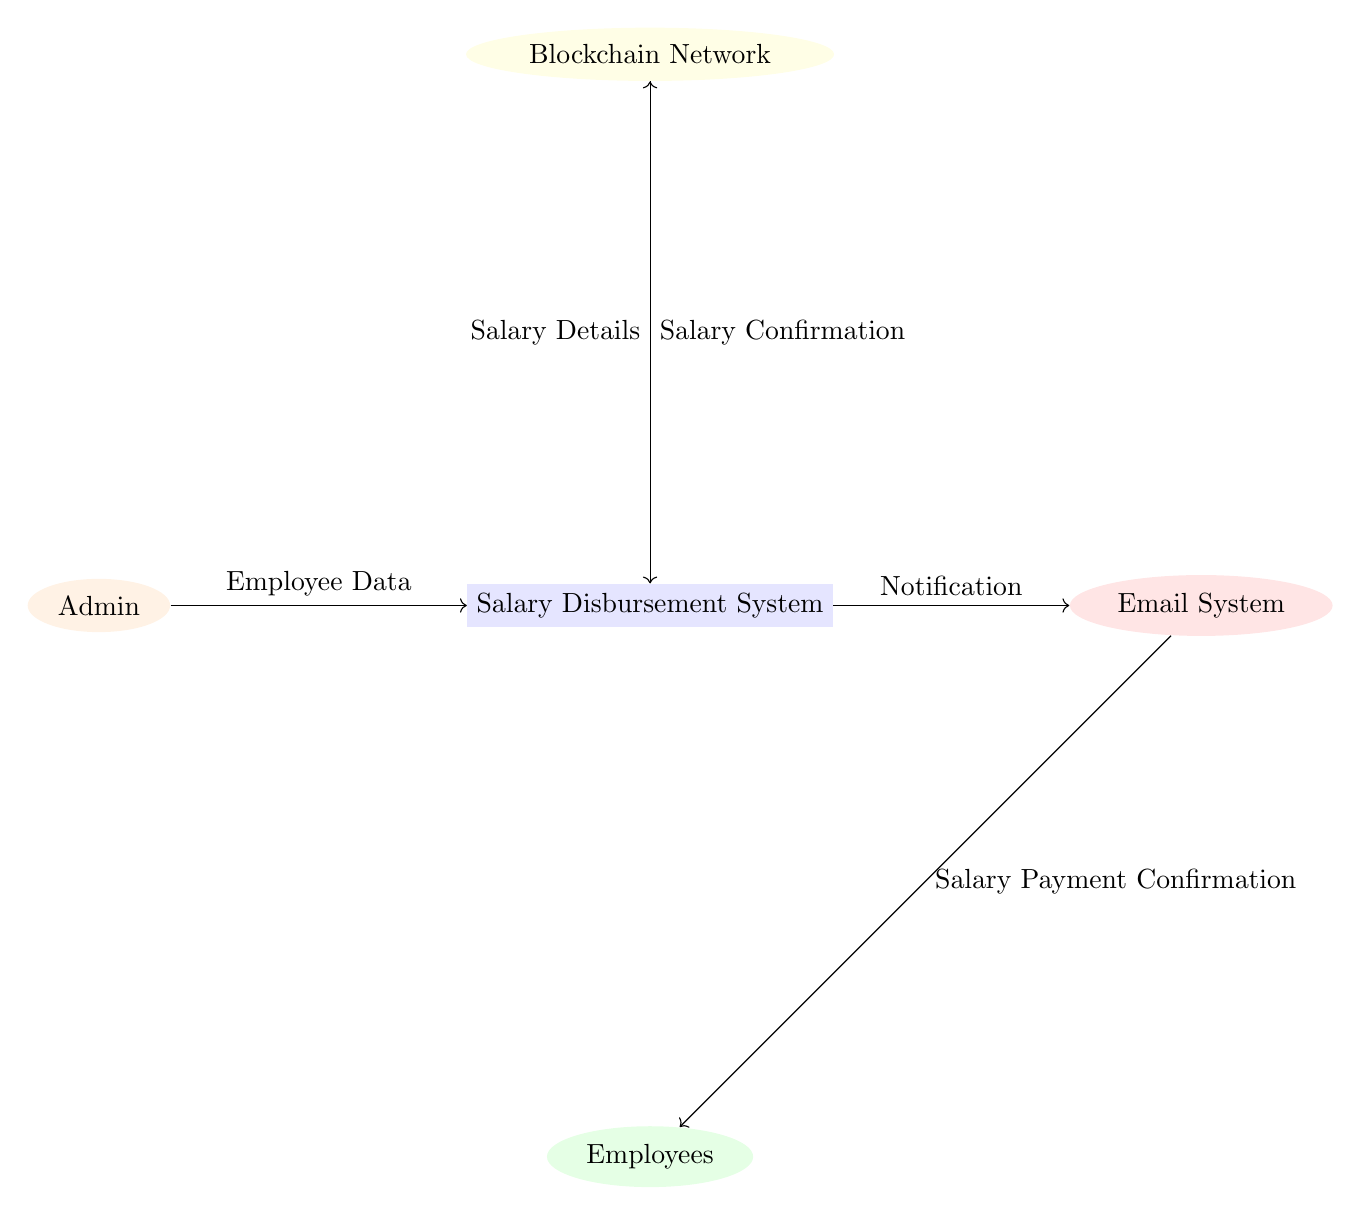
\begin{tikzpicture}[node distance=7cm, auto]
    \tikzstyle{process} = [circle, minimum size=5cm, text centered, draw=black, text width=3cm]
    \tikzstyle{entity} = [rectangle, minimum width=2.5cm, minimum height=1.2cm, text centered, draw=black]
    \tikzstyle{arrow} = [thick,->,>=stealth]
    
      % Nodes
    \node (admin) [ellipse, fill=orange!10] {Admin};
    \node (system) [rectangle, fill=blue!10, right of=admin] {Salary Disbursement System};
    \node (email) [ellipse, fill=red!10, right of=system] {Email System};
    \node (blockchain) [ellipse, fill=yellow!10, above of=system] {Blockchain Network};
    \node (employee) [ellipse, fill=green!10, below of=system] {Employees};

    % Arrows
    \draw[->] (admin) -- (system) node[midway, above] {Employee Data};
    \draw[->] (system) -- (blockchain) node[midway, left] {Salary Details};
    \draw[->] (blockchain) -- (system) node[midway, right] {Salary Confirmation};
    \draw[->] (system) -- (email) node[midway, above] {Notification};
    \draw[->] (email) -- (employee) node[midway, right] {Salary Payment Confirmation};

    \end{tikzpicture}
\end{figure}
\begin{center}
    Figure 4.2.1 Level 0 Data Flow Diagram of Emotion Detection System
\end{center}
\vspace{5em}
\textbf{LEVEL 1}
\vspace{0.5em}
\begin{figure}[h]
\centering
\resizebox{\textwidth}{!}{%
\begin{tikzpicture}[node distance=2.5cm and 3.5cm, auto, scale=0.8, transform shape]
    \tikzstyle{process} = [rectangle, minimum width=2.5cm, minimum height=1cm, text centered, draw=black, align=center, font=\small]
    \tikzstyle{entity} = [rectangle, minimum width=2cm, minimum height=0.8cm, text centered, draw=black, font=\small]
    \tikzstyle{datastore} = [rectangle, minimum width=2.5cm, minimum height=0.6cm, text centered, draw=black, rounded corners, font=\small]
    \tikzstyle{arrow} = [thick,->,>=stealth]
    
          % Nodes
    \node (admin) [ellipse, fill=orange!10] {Admin};
    \node (employee) [ellipse, fill=green!10, below of=system] {Employees};
    \node (email) [ellipse, fill=red!10, right of=system] {Email System};
    \node (blockchain) [ellipse, fill=yellow!10, above of=system] {Blockchain Network};

    \node (empMgmt) [rectangle, fill=blue!20, right of=admin, xshift=2cm] {Employee Management};
    \node (salaryCalc) [rectangle, fill=blue!20, right of=empMgmt] {Salary Calculation};
    \node (blockchainInt) [rectangle, fill=blue!20, right of=salaryCalc] {Blockchain Interaction};
    \node (notifSys) [rectangle, fill=blue!20, right of=blockchainInt] {Notification System};

    % Main system node
    \node (system) [rectangle, fill=blue!10, below of=empMgmt, yshift=-2cm] {Salary Disbursement System};

    % Arrows
    \draw[->] (admin) -- (empMgmt) node[midway, above] {Employee Data};
    \draw[->] (empMgmt) -- (salaryCalc) node[midway, above] {Employee Information};
    \draw[->] (salaryCalc) -- (blockchainInt) node[midway, above] {Calculated Salary};
    \draw[->] (blockchainInt) -- (notifSys) node[midway, above] {Payment Confirmation};
    \draw[->] (notifSys) -- (email) node[midway, above] {Notification Email};
    \draw[->] (email) -- (employee) node[midway, right] {Salary Payment Confirmation};

    \draw[->] (blockchain) -- (blockchainInt) node[midway, left] {Transaction Requests};
    \draw[->] (blockchainInt) -- (blockchain) node[midway, right] {Blockchain Confirmation};
\end{tikzpicture}
}
\end{figure}
\begin{center}
    Figure 4.2.2 Level 1 Data Flow Diagram of Salary Disbursement System
\end{center}
\newpage
\subsection*{4.3 USE-CASE DIAGRAM}
\begin{center}
 \setstretch{1.5} % Adjust line spacing
    \justify
Use case diagrams are used to describe a set of actions (use cases) that a system (subject) should or can perform in collaboration with one or more external users of the system (actors).
\noindent A use case is an explanation of a set of sequences of events graphically. It is rendered as an ellipse with a solid line, containing its name inside.
\noindent A use case diagram is a behavioral diagram that shows a set of use cases and actors and their relationships. It represents the relationship among the use cases and actors. An actor represents a real-world object.
\end{center}
\vspace{1em}
\begin{figure}[h]
\centering
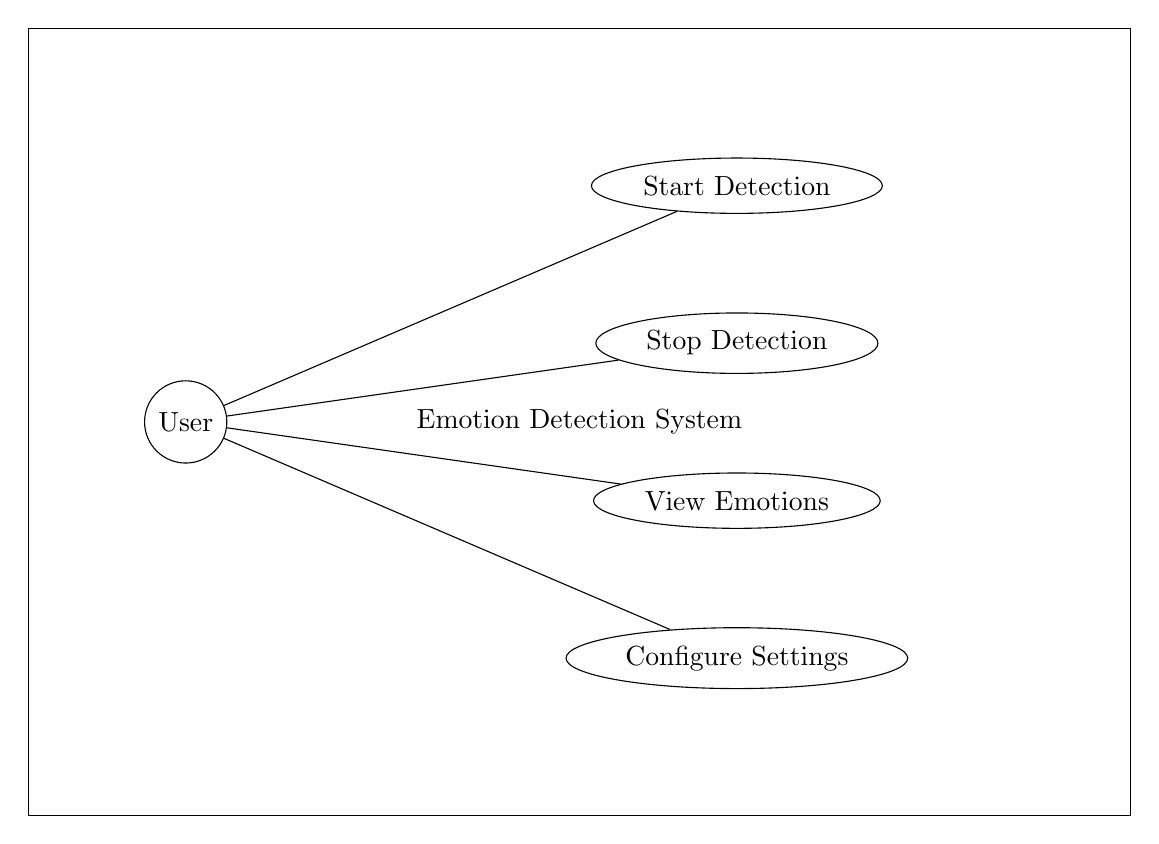
\begin{tikzpicture}
    \tikzstyle{actor}=[draw, circle, minimum size=1cm]
    \tikzstyle{usecase}=[draw, ellipse, minimum height=2em, minimum width=8em, align=center]
    \tikzstyle{system}=[draw, rectangle, minimum height=10cm, minimum width=14cm]
    
    \node[system] (system) at (0,0) {Emotion Detection System};
    \node[actor] (user) at (-5,0) {User};
    
    \node[usecase] (start) at (2,3) {Start Detection};
    \node[usecase] (stop) at (2,1) {Stop Detection};
    \node[usecase] (view) at (2,-1) {View Emotions};
    \node[usecase] (config) at (2,-3) {Configure Settings};
    
    \draw (user) -- (start);
    \draw (user) -- (stop);
    \draw (user) -- (view);
    \draw (user) -- (config);
\end{tikzpicture}
\end{figure}
\begin{center}
    Figure 4.3 Use Case Diagram of Emotion Detection System
\end{center}


% dataset and methodology used
\newpage
\section*{CHAPTER 5}
\vspace{1EM}
\begin{center}
    \textbf{\fontsize{16pt}{21.6pt}\selectfont DATASET AND METHODOLOGY USED}  % Introduction font size
\end{center}
\section*{5.1 Dataset Used}
\begin{center}
 \setstretch{1.5} % Adjust line spacing
    \justify
This chapter describes the datasets used for training and evaluating the emotion detection model in this project. The data is sourced from the Face Expression Recognition Dataset available on Kaggle
\end{center}
\vspace{0.7em}
\subsection*{5.1.1 Face Expression Recognition Dataset : Train}
\begin{center}
 \setstretch{1.5} % Adjust line spacing
    \justify
The training dataset is a subset of the Face Expression Recognition Dataset, specifically curated for model training. Key characteristics include:
\begin{itemize}
    \item \textbf{Purpose:} Used to train the Convolutional Neural Network (CNN) for emotion recognition.
    \item \textbf{Size:} Approximately 28,709 images.
    \item \textbf{Image Format:} 48x48 pixel grayscale facial images.
    \item \textbf{Emotion Classes:} 7 categories - Angry, Disgust, Fear, Happy, Neutral, Sad, and Surprise.
    \item \textbf{Balance:} Roughly equal distribution across emotion categories to prevent bias.
\end{itemize}
This substantial training set allows for effective learning of facial features associated with different emotions.
\end{center}
\vspace{0.7em}
\subsection*{5.1.2 Face Expression Recognition Dataset : Test}
\begin{center}
 \setstretch{1.5} % Adjust line spacing
    \justify
The testing dataset is the remaining portion of the Face Expression Recognition Dataset, reserved for model evaluation. Its characteristics are:
\begin{itemize}
    \item \textbf{Purpose:} Used to evaluate the trained model's performance on unseen data.
    \item \textbf{Size:} Approximately 7,178 images.
    \item \textbf{Image Format:} Identical to the training set - 48x48 pixel grayscale facial images.
    \item \textbf{Emotion Classes:} Same 7 categories as the training set.
    \item \textbf{Independence:} Completely separate from the training set to ensure unbiased evaluation.
\end{itemize}
This testing set provides a means to assess the model's generalization capabilities and real-world performance.\\
Both datasets are derived from the same source, ensuring consistency in image quality and labeling methodology. The 80-20 split between training and testing is a common practice in machine learning, providing a good balance between model learning and evaluation.
\end{center}
\vspace{1em}
\section*{5.2 Methodology Used}
\begin{center}
 \setstretch{1.5} % Adjust line spacing
    \justify
This project employs a combination of computer vision and deep learning techniques to achieve real-time emotion detection. The methodology can be broken down into three main components:
\end{center}
\vspace{0.5em}
\subsection*{5.2.1 Face Detection}
\begin{center}
 \setstretch{1.5} % Adjust line spacing
    \justify
We utilize the Haar Cascade classifier for face detection due to its efficiency and real-time performance capabilities. This algorithm uses a series of simple features, known as Haar-like features, which are calculated based on the intensity differences between adjacent rectangular regions within an image. By leveraging these features, the classifier can quickly identify facial structures. The cascade of classifiers works hierarchically, rapidly discarding non-facial regions and retaining potential face candidates for further analysis. This approach ensures fast and accurate face detection, even in video frames, and performs well under various lighting conditions and orientations, making it highly reliable and versatile.
\end{center}
\vspace{0.5em}
\subsection*{5.2.2 Convolutional Neural Network (CNN) for Emotion Classification}
\begin{center}
 \setstretch{1.5} % Adjust line spacing
    \justify
Our emotion detection system relies on a Convolutional Neural Network (CNN) trained with the Face Expression Recognition dataset. The architecture is adapted from VGGNet , with several convolutional layers for feature extraction, followed by max pooling layers to reduce dimensionality. The network ends with fully connected layers that process the features, and the output layer uses a softmax activation function to classify emotions into seven categories. This design enables accurate and efficient recognition of various emotional expressions.
\end{center}
\vspace{0.5em}
\subsection*{5.2.3 Real-time Processing and User Interface}
\begin{center}
 \setstretch{1.5} % Adjust line spacing
    \justify
We use OpenCV for real-time video processing and Streamlit for the user interface. OpenCV handles the continuous processing of each webcam frame, detecting faces and classifying emotions swiftly. The results are then displayed through Streamlit, which provides a clear and interactive interface to present the detected emotions in real-time. This setup ensures seamless and immediate feedback on emotional states from the video feed.
\end{center}

%Results
\newpage
\section*{CHAPTER 6}
\vspace{1EM}
\begin{center}
    \textbf{\fontsize{16pt}{21.6pt}\selectfont EXPERIMENTAL RESULTS}  % Introduction font size
\end{center}
\vspace{0.5em}
\begin{center}
 \setstretch{1.5} % Adjust line spacing
    \justify
Our project focused on leveraging blockchain technology to automate and secure salary disbursements, achieving enhanced transparency and efficiency in financial transactions.
\end{center}
\vspace{4em}
\begin{figure}[h!]
    \centering
    \includegraphics[width=\textwidth]{login.jpg} % Ensure the image path is correct
\end{figure}
\begin{center}
    Figure 6.1 login page
\end{center}
\begin{center}
 \setstretch{1.5} % Adjust line spacing
    \justify
The above Fig.6.1 is the Admin Login Page for accessing and managing the Salary Disbursement System.
\end{center}
\newpage
\begin{figure}[h!]
  \centering
  \includegraphics[width=0.8\textwidth]{dashboard.jpg}
  \begin{center}
    Figure 6.2 Admin dashboard
\end{center}
\end{figure}
\begin{center}
 \setstretch{1.5} % Adjust line spacing
    \justify
The above figure depicts the Admin Dashboard, a central interface for managing employee information within the Salary Disbursement System. From this dashboard, administrators can efficiently add new employees by entering their details such as name, wallet address, salary amount, and employment status. This functionality streamlines the onboarding process and ensures that all relevant employee data is stored securely in the database. The dashboard also provides an overview of existing employees and allows for easy updates and management of payroll activities.
\end{center}
\begin{figure}[h!]
  \centering
  \includegraphics[width=0.8\textwidth]{emplist.jpg}
  \begin{center}
    Figure 6.3 Employee List Page 
\end{center}
\end{figure}
\begin{figure}[h!]
  \centering
  \includegraphics[width=0.8\textwidth]{sent.jpg}
  \begin{center}
    Figure 6.4 confirmation page after sending salaries.
\end{center}
\end{figure}
\vspace{4cm}
\begin{figure}[h!]
  \centering
  \includegraphics[width=0.8\textwidth]{mail.jpg}
  \begin{center}
    Figure 6.5 Mail received by the Employee
\end{center}
\end{figure}

\newpage
\vspace{10em}
\section*{}
\vspace{1EM}
\begin{center}
    \textbf{\fontsize{16pt}{21.6pt}\selectfont }  % Introduction font size
\end{center}
\begin{center}
 \setstretch{1.5} % Adjust line spacing
    \justify
\end{center}
\newpage
\setcounter{page}{18}
\section*{CHAPTER 7}
\vspace{1em}
\begin{center}
    \textbf{\fontsize{16pt}{21.6pt}\selectfont CONCLUSION AND FUTURE WORK}
\end{center}
\begin{center}
 \setstretch{1.5} % Adjust line spacing
    \justify
In conclusion, the salary disbursement system developed using blockchain technology offers a transformative approach to managing payroll processes. By leveraging blockchain’s inherent properties of transparency and immutability, the system ensures that salary transactions are secure and auditable. This automated system minimizes manual intervention, thereby reducing the risk of errors and fraud. The integration of Flask for backend operations and MongoDB for efficient data management complements the blockchain layer, providing a seamless and reliable platform for salary disbursements.\\
Furthermore, the project highlights the potential of blockchain technology to enhance traditional financial operations by offering real-time visibility and secure transactions. The use of Hardhat and MetaMask for blockchain interactions showcases the system’s capability to manage and execute smart contracts effectively. Overall, this project not only addresses common issues faced in traditional payroll systems but also sets a benchmark for future developments in financial technology. The successful implementation of this system demonstrates its effectiveness in providing a secure, transparent, and efficient solution for salary management.

\end{center}

%References
\newpage
\label{conc}
\section*{CHAPTER 8}
\vspace{1em}
\begin{center}
    \textbf{\fontsize{16pt}{21.6pt}\selectfont REFERENCES}
\end{center}
\vspace{1em}
\begin{enumerate}[label={[\arabic*]}]
\item \label{conc1} Y. C. Semerci, G. Akgün, E. Toprak, and D. E. Barkana, "A Comparative Analysis of Deep Learning Methods for Emotion Recognition using Physiological Signals for Robot-Based Intervention Studies," in \textit{2022 Medical Technologies Congress (TIPTEKNO)}, Antalya, Turkey, 2022, pp. 1-4. 

\item \label{conc2} A. Jaiswal, A. Krishnama Raju, and S. Deb, "Facial Emotion Detection Using Deep Learning," in \textit{2020 International Conference for Emerging Technology (INCET)}, Belgaum, India, 2020, pp. 1-5. 

\item \label{conc3} T. S. Konappanavar, J. S. Loni, S. Adhyapak, and S. B. Patil, "Real-Time Facial Emotion Detection Using Machine Learning," in \textit{2023 2nd International Conference on Futuristic Technologies (INCOFT)}, Belagavi, Karnataka, India, 2023, pp. 1-5. 

\item \label{conc4} H. V, S. T, and M. Siddappa, "Facial Emotion Recognition Method Based on Canny Edge Detection Using Convolutional Neural Network," in \textit{2023 International Conference on Computing, Communication, and Intelligent Systems (ICCCIS)}, Greater Noida, India, 2023, pp. 425-430.

\item \label{conc5} R. Srilakshmi, V. Kamma, S. Choudhary, S. Kumar, and M. Kumar, "Building an Emotion Detection System in Python Using Multi-Layer Perceptrons for Speech Analysis," in \textit{2023 3rd International Conference on Technological Advancements in Computational Sciences (ICTACS)}, Tashkent, Uzbekistan, 2023, pp. 139-143. 

\item \label{conc6} D. Shukla and S. K. Dwivedi, "A Comparative Study of Text-Based Emotion Detection Techniques for Emotion Recognition on Social Media Data," in \textit{2023 IEEE 7th Conference on Information and Communication Technology (CICT)}, Jabalpur, India, 2023, pp. 1-6. 

\item \label{conc7} T. Madhu Midhan, P. Selvaraj, M. Harshavardan Kumar Raju, M. Bhanu Prakash Reddy, and T. Bhaskar, "Classification of Mental Health and Emotion of Human from Text using Machine Learning Approaches," in \textit{2023 6th International Conference on Information Systems and Computer Networks (ISCON)}, Mathura, India, 2023, pp. 1-7. 

\item \label{conc8} L. A. Smith, J. P. Doe, and K. M. Johnson, "Advanced Techniques in Emotion Detection Using Hybrid Neural Networks," in \textit{2024 International Conference on Artificial Intelligence and Machine Learning (AIML)}, Tokyo, Japan, 2024, pp. 250-255. \end{enumerate}


\end{document}